%Fiquemos com Deus e Nossa Senhora!
%Sao Jose de Cupertino rogai por nos!!
% ### Uses XeLaTeX ### %
% ### Needs beamer-master ### %
\documentclass[aspectratio=169]{beamer} %. Aspect Ratio 16:9

\usetheme{AI2} % beamerthemeSprace.sty
\usepackage[portuguese]{babel}
\usepackage[utf8]{inputenc}
\usepackage[T1]{fontenc}
\usepackage{ragged2e,gensymb}

\DeclareMathOperator*{\argmin}{arg\,min}
\DeclareMathOperator*{\argmax}{arg\,max}
\DeclareMathOperator{\sign}{sgn}

% DATA FOR FOOTER
\date{2021}
\title{- Floresta de Caminhos Ótimos}
\author{João Paulo Papa}
\institute{Advanced Institute for Artificial Intelligence (AI2)}

\begin{document}
% ####################################
% FIRST SLIDE 						:: \SliTit{This is the Title of the Talk}{A. B. Name}{Sprace}
% SUB-TITLE SLIDE 					:: \SliSubTit{<title>}{<explanation}
% SUB-SUB-TITLE SLIDE				:: \SliSubSubTit{<title>}{<explanation}
% SLIDE WITH TITLE 					:: \SliT{Title}{Content}
% SLIDE NO TITLE 						:: \Sli{Content} 
% SLIDE DOUBLE COLUMN WITH TITLE 	:: \SliDT{Title}{First Column}{Second Column}
% SLIDE DOUBLE COLUMN NO TITLE 		:: \SliD{First Column}{Second Column}
% SLIDE ADVANCED WITH TITLE 			:: \SliAdvT{Title}{Content}
% SLIDE ADVANCED NO TITLE 			:: \SliAdv{Content}
% SLIDE ADVANCED DOUBLE WITH TITLE 	:: \SliAdvDT{Title}{First Column}{Second Column}
% SLIDE ADVANCED DOUBLE NO TITLE 	:: \SliAdvD{First Column}{Second Column}
% SLIDE BLACK						:: \Black{ <Content> }
% SLIDE WHITE						:: \White{ <Content> }
% ITEMIZATION 						:: \begin{itemize}  \iOn{First} \iTw {Second} \iTh{Third} \end{itemize}
% COMMENT TEXT				 		:: \note{<comment>}
% SECTION 							:: \secx{Section} | \secxx{Sub-Section}
% BOLD SPRACE COLOR				:: \bfs{<text>}
% TABLE OF CONTENT					:: \tocitem{<title>}{<content>}
% LEFT ALIGN EQUATION				:: \begin{flalign*}  & <equation> &   \end{flalign*}
% CENTER ALIGN EQUATION	S			:: \begin{gather*} <equations>  \end{gather*}
% SLASH								:: \slashed{<>}
% BAR								:: \barr{<letter>} instead of \bar{<letter>}
% THEREFORE						:: use \portanto (larger and bold}
% 2 or 3 MATH SYMBOLS				:: \overset{<up>}{<down>} &  \underset{<below>}{\overset{<above>}{<middle>}}  
% INSERT TEXT IN FORMULA			:: \ins{<text>}
% EXERCISE							:: \exe{<exercise #>}{<exercise text>}
% SUGGESTED READING BOX			:: \sug{<references>}
% CITATION							:: \cittex{<citation>}
% CITATION DOUBLE COLUMN 			:: \cittexD{<citation>}
% TEXT POSITION						:: \texpos{<Xcm>}{<Ycm>}{<text>} origin = center of slide : x right | y down
% REFERENCE AT BOTTOM  S/D SLIDE		:: \refbotS{<reference>} \refbotD{<reference>}
% HIDDEN SLIDE						:: \hid
% COLOR BOX 						:: \blu{blue} + \red{rec} + \yel{yellow} + \gre{green} + \bege{beige}
% FRAME 							:: \fra{sprace} \frab{blue} \frar{red} + \fray{yellow} + \frag{green}		
% FIGURE 							:: \img{X}{Y}{<scale>}{Figure.png} 
% FIGURE							:: \includegraphics[scale=<scale>]{Figures/.png}
% FIGURE DOUBLE SLIDE NO TITLE		::  \img{-4}{0.5}{<scale>}{Figure.png} % Image 1st half
%									::  \img{4}{0.5}{<scale>}{Figure.png} % Image 2nd half
% FIGURE DOUBLE SLIDE WITH TITLE		::  \img{-4}{0}{<scale>}{Figure.png} % Image 1st half
%									::  \img{4}{0}{<scale>}{Figure.png} % Image 2nd half
% INCLUDING SWF (Flash)				:: \usepackage{media9} and \includemedia >> USE ACROBAT <<
%%%%%%%%%%%%%%%%%%%%%%%%%%%%%%%%%%%%%%%%%%%%%%%%%%
% ###############################################################################
% FIRST SLIDE
\SliTit{{\LARGE Floresta de Caminhos Ótimos}}{Advanced Institute for Artificial Intelligence -- AI2}{https://advancedinstitute.ai}
%%%%%%%%%%%%%%%%%%%%%%%%%%%%%%%%%%%%%%%%%%%%%%%%%%
% ###############################################################################
% SLIDE SUB-TITLE
%\SliSubTit{Sub-Title}{Description}{}
%%%%%%%%%%%%%%%%%%%%%%%%%%%%%%%%%%%%%%%%%%%%%%%%%%
% ###############################################################################
%\SliSubSubTit{Sub-Sub-Title}{Description}
 %%%%%%%%%%%%%%%%%%%%%%%%%%%%%%%%%%%%%%%%%%%%%%%%%%


\SliT{Introdução}{

\justifying Existe um conjunto de abordagens que tratam o problema de classificação de padrões como sendo uma tarefa de particionamento em \textbf{grafos}. No entanto, o que seriam esses chamados grafos? Grafos podem ser entendidos como estruturas de dados que são compostas por \textbf{vértices} e \textbf{arestas} e que, dependendo de suas propriedades, podem modelar diferentes problemas.

\begin{center}
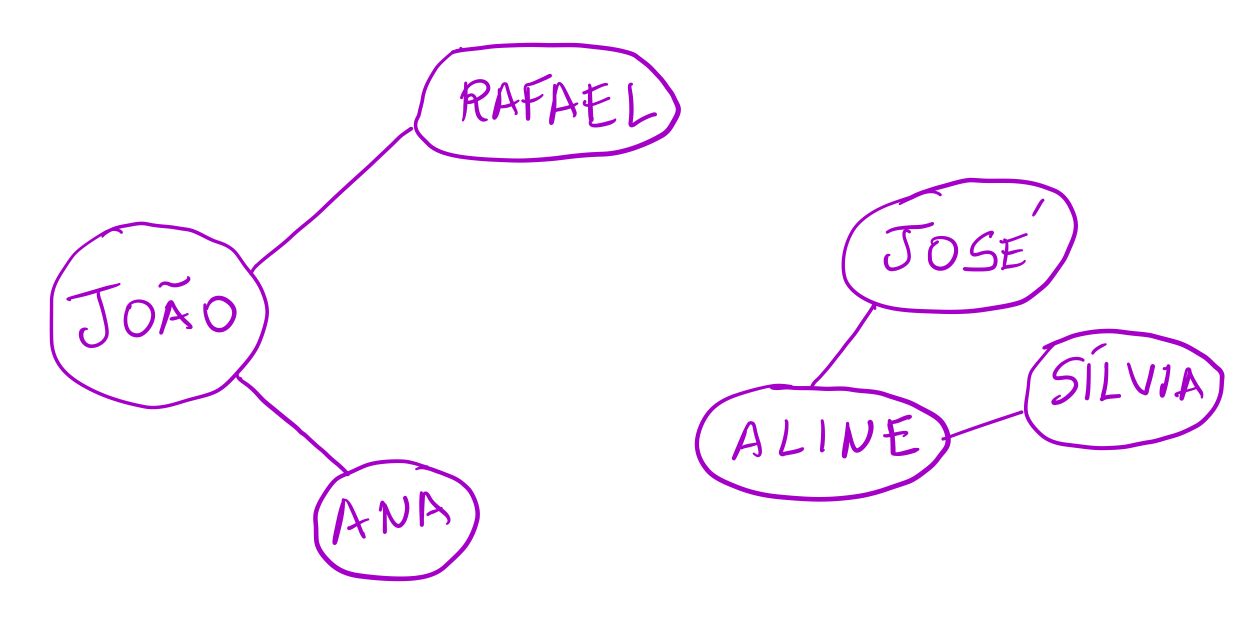
\includegraphics[scale=0.17]{./figs/OPF_Fig1.png}
\end{center}
}

\Sli{
\justify A Teoria dos Grafos é uma área que estuda o comportamento dos grafos e propõe análises teóricas e desenvolvimento de algoritmos para eles. Matematicamente falado, um grafo é definido como $G=({\cal V},{\cal E})$, em que ${\cal V}$ denota o conjunto de vértices (nós) e ${\cal E}$ corresponde ao conjunto de arestas (pares de nós). Vejamos o exemplo abaixo.

\begin{minipage}{0.43\textwidth}
\begin{center}
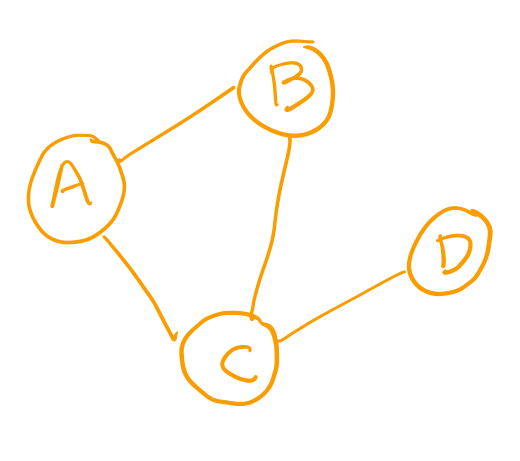
\includegraphics[scale=0.21]{./figs/OPF_Fig2.png}
\end{center}
\end{minipage}%%% to prevent a space
\begin{minipage}{0.49\textwidth}
Neste caso, temos que $G=({\cal V},{\cal E})$, em que ${\cal V}=\{A,B,C,D\}$ e ${\cal E}=\{(A,B),(A,C),(B,C),(C,D)\}$. Note que a \textbf{relação de adjacência} é \textbf{simétrica}, ou seja, as arestas $(A,B)$ e $(B,A)$ são iguais neste caso.
\null
\par\xdef\tpd{\the\prevdepth}
\end{minipage}
}

\Sli{
\justify Assim sendo, problemas que podem ser modelados como sendo grafos são beneficiados por inúmeros algoritmos já desenvolvidos para diversas aplicações. Grafos podem ser classificados de acordo com sua topologia e relação de adjacência, principalmente. Com relação à topologia, podemos dividir os grafos em:

\begin{center}
\begin{tabular}{cc}
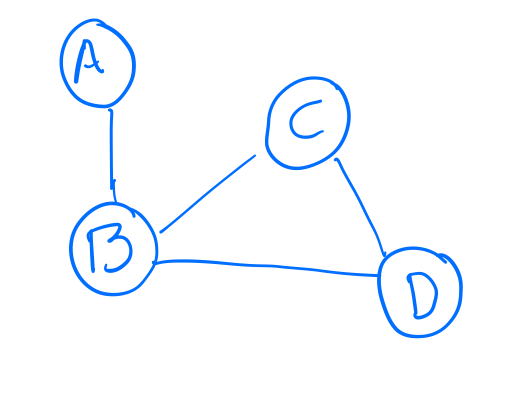
\includegraphics[scale=0.19]{./figs/OPF_Fig3.png} &
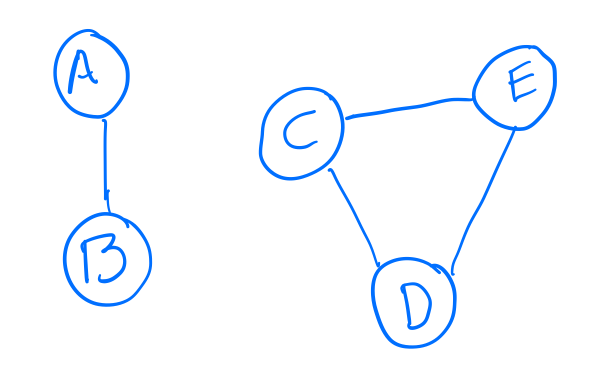
\includegraphics[scale=0.19]{./figs/OPF_Fig4.png} \\
Grafo conexo & Grafo desconexo\\	
\end{tabular}
\end{center}
}

\Sli{
Ou ainda em:

\begin{center}
\begin{tabular}{ccc}
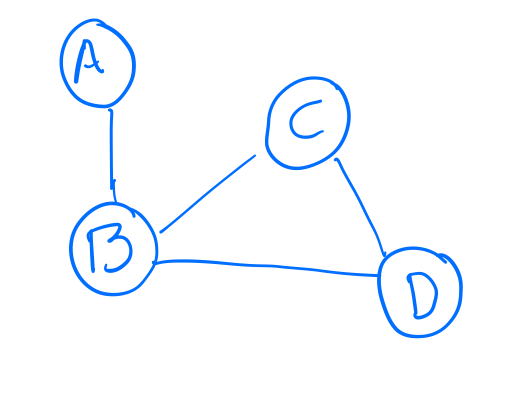
\includegraphics[scale=0.19]{./figs/OPF_Fig3.png} &
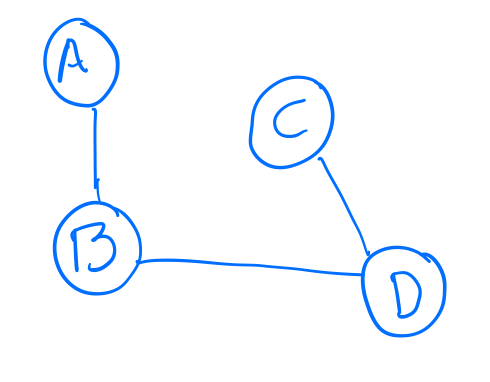
\includegraphics[scale=0.19]{./figs/OPF_Fig5.png} &
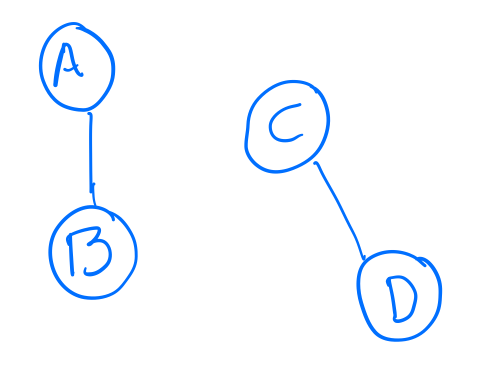
\includegraphics[scale=0.19]{./figs/OPF_Fig6.png}\\
Grafo cíclico & Grafo acíclico (árvore) & Floresta\\	
\end{tabular}
\end{center}
}

\Sli{
De acordo com a sua relação de adjacência, podemos classificar os grafos em:

\begin{center}
\begin{tabular}{cc}
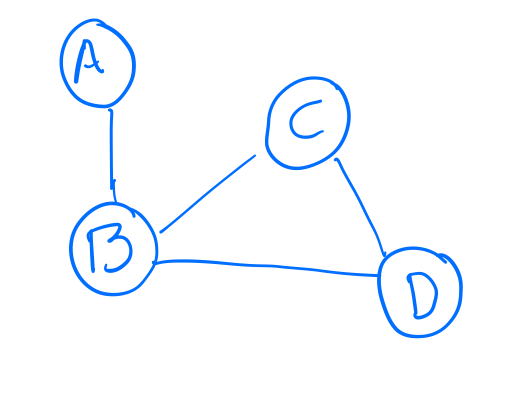
\includegraphics[scale=0.19]{./figs/OPF_Fig3.png} &
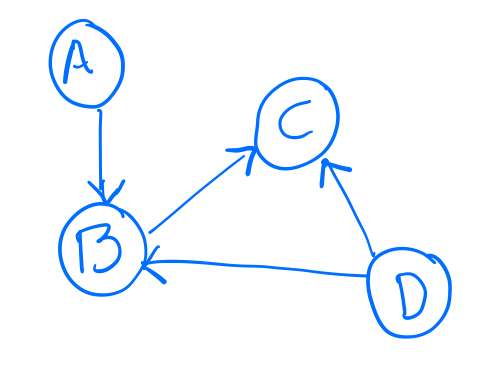
\includegraphics[scale=0.19]{./figs/OPF_Fig7.png}\\
Grafo não direcionado & Grafo direcionado\\
\end{tabular}
\end{center}
}

\Sli{
\justify Grafos são, de maneira geral, definidos como sendo conjuntos de vértices e arestas. Desta forma, conseguimos classificá-los, ainda, de acordo com seus subconjuntos: \textbf{subgrafo gerador} e \textbf{subgrafo gerado}.

\begin{center}
\begin{tabular}{ccc}
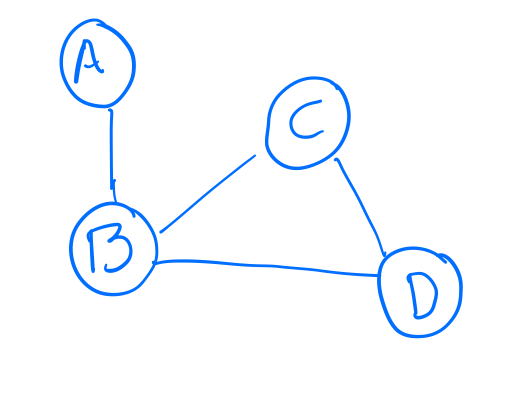
\includegraphics[scale=0.19]{./figs/OPF_Fig3.png} &
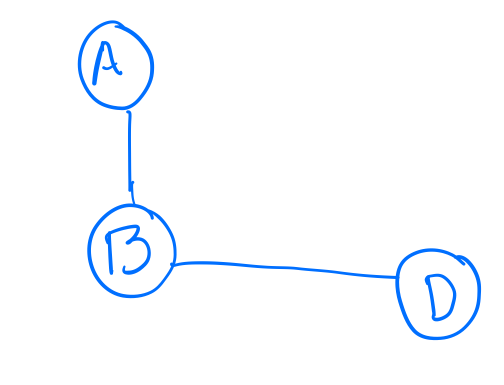
\includegraphics[scale=0.19]{./figs/OPF_Fig8.png} &
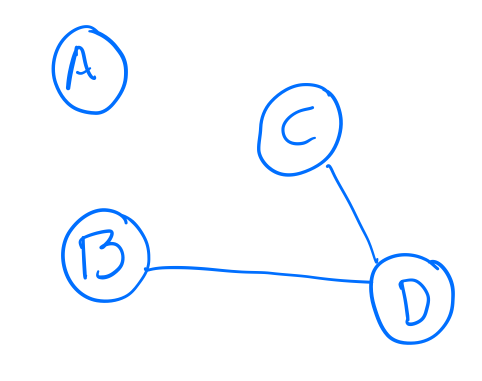
\includegraphics[scale=0.19]{./figs/OPF_Fig9.png}\\
Grafo original & Subgrafo gerado & Subgrafo gerador\\	
\end{tabular}
\end{center}
}

\Sli{
\justify Um grafo é dito ser completo quando todos os pares de nós estão conectados. Uma família bastante conhecida de grafos que obedece à esta propriedade é conhecida por $K_z$, em que $z$ denota o número de nós.

\begin{center}
\begin{tabular}{ccc}
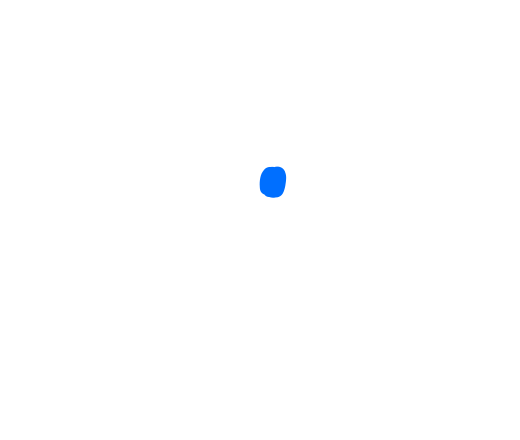
\includegraphics[scale=0.19]{./figs/OPF_Fig14.png} &
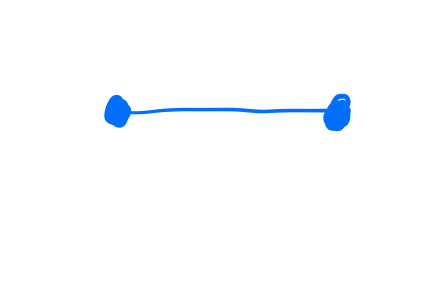
\includegraphics[scale=0.19]{./figs/OPF_Fig15.png} &
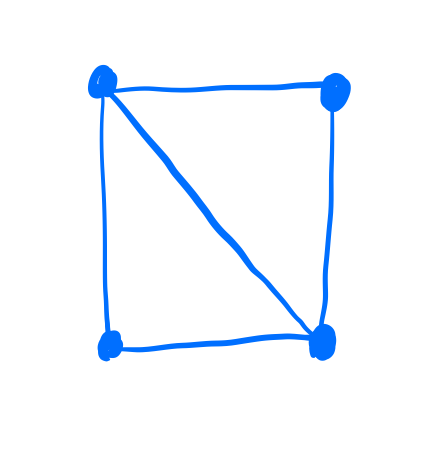
\includegraphics[scale=0.19]{./figs/OPF_Fig16.png}\\
$K_1$ (grafo trivial) & $K_2$ & $K_4$\\
\end{tabular}
\end{center}
}

\Sli{
\justify Grafos podem ser ainda \textbf{ponderados} em suas arestas (distâncias entre cidades, por exemplo). Desta forma, temos que nosso grafo pode ser definido como segue: $G=({\cal V},{\cal E},w)$, em que $w:{\cal V}\times{\cal V}\rightarrow\mathbb{R}$ é a função que associa pesos às arestas. De acordo com essa definição, temos um importante tipo de grafo chamado de \textbf{árvore geradora mínima}, do inglês \emph{minimum spanning tree} - MST, que é um subgrafo gerador, do tipo árvore, cujo somatório dos pesos das arestas é \textbf{mínimo}.

\begin{center}
\begin{tabular}{cc}
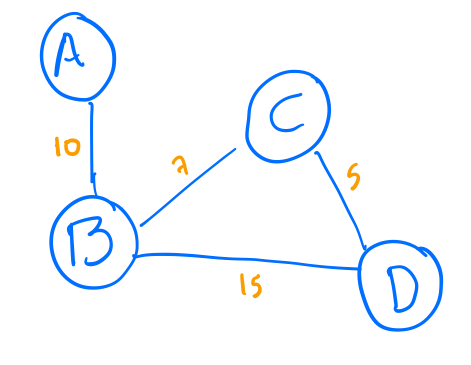
\includegraphics[scale=0.19]{./figs/OPF_Fig10.png} &
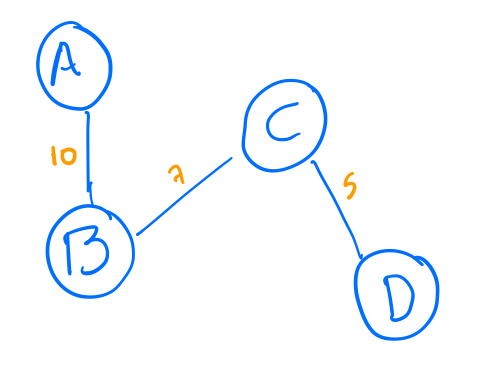
\includegraphics[scale=0.19]{./figs/OPF_Fig11.png}\\
Grafo original & MST\\	
\end{tabular}
\end{center}
}

\Sli{
\justify A técnica Floresta de Caminhos Ótimos, do inglês \emph{Optimum-Path Forest} - OPF, visa modelar o problema de classificação das amostras como sendo uma tarefa de particionamento de um grafo em grupos de amostras com o mesmo rótulo. Neste sentido, as amostras do conjunto de dados correspondem aos nós do grafo e as arestas são definidas por alguma relação de adjacência escolhida previamente.

\justify \underline{Definição do problema:} dados um conjunto de treinamento rotulado e com $m$ amostras, ou seja, ${\cal X}^1 = \{(\boldsymbol{x}_1,y_1),(\boldsymbol{x}_2,y_2),\ldots,(\boldsymbol{x}_m,y_m)\}$ e um grafo $G=({\cal V},{\cal E},w)$, nosso objetivo é então particionar $G$ em grupos de amostras com o mesmo rótulo. Temos que ${\cal V}=\{\boldsymbol{x}_1,\boldsymbol{x}_2,\ldots,\boldsymbol{x}_m\}$, ${\cal E}$ deve ser escolhido de alguma forma que satisfaça o seu problema e $w$ é geralmente escolhido como uma função distância entre duas amostras, ou seja, $w(\boldsymbol{x}_i,\boldsymbol{x}_j)$ calcula a distância entre os nós (amostras) $\boldsymbol{x}_i$ e $\boldsymbol{x}_j$. De maneira geral, o classificador OPF usa a distância euclidiana para este fim.
}

\Sli{
\justify Como particionar o conjunto de dados de treinamento em grupos? O classificador OPF usa a ideia de \textbf{competição} entre alguns nós denominados de \textbf{protótipos}, os quais tentam conquistar as demais amostras do conjunto de treinamento atribuindo \textbf{melhores} custos à elas por meio de \textbf{caminhos de custo ótimo}. O que são esses caminhos?

\begin{center}
\begin{tabular}{ccc}
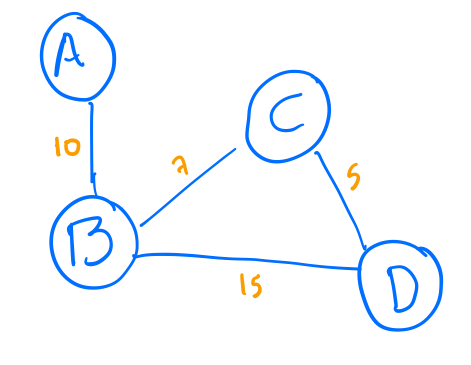
\includegraphics[scale=0.19]{./figs/OPF_Fig10.png} &
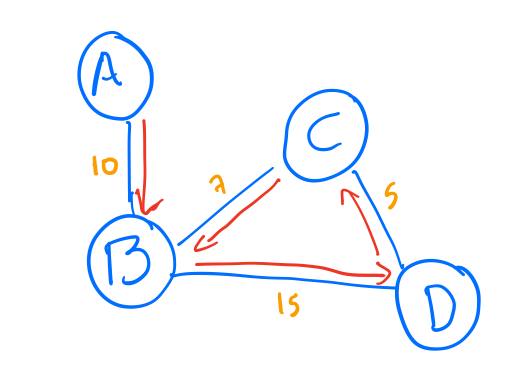
\includegraphics[scale=0.19]{./figs/OPF_Fig12.png} &
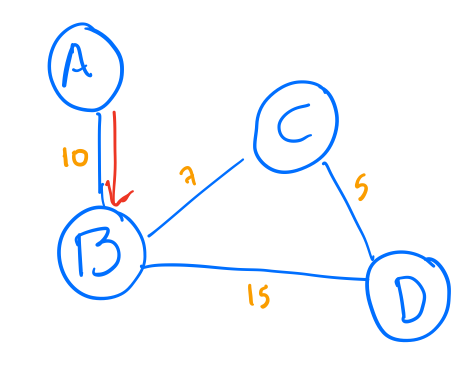
\includegraphics[scale=0.19]{./figs/OPF_Fig13.png}\\
Grafo original & Passeio & Caminho\\
& $\pi_B=\langle A,B,D,C,B\rangle$ & $\pi_B=\langle A,B\rangle$
\end{tabular}
\end{center}
}

\Sli{
\justify O classificador OPF opera em duas etapas, como de costume com outros classificadores, isto é, treinamento e teste. A etapa de treinamento é responsável por particionar o grafo em grupos de amostras com o mesmo rótulo (árvores de caminhos ótimos, do inglês \emph{optimum-path trees} - OPTs), enquanto que a etapa de teste associa, à cada amostra do conjunto de teste, a sua amostra de treinamento mais \textbf{fortemente conexa}.

\justify A etapa de treinamento é composta por três passos:
\begin{itemize}
	\item Criação do grafo por meio da escolha da \underline{relação de adjacência}.
	\item Escolha das amostras \underline{protótipos} e da \underline{função de custo}.
	\item Processo de \underline{conquista}.
\end{itemize}
}

\Sli{
\justify Dependendo da relação de adjacência escolhida, metodologia para estimar protótipos e função de custo, diferentes classificadores OPF podem ser obtidos. Iremos abordar a primeira versão proposta, que possui as seguintes características:

\begin{itemize}
	\item Relação de adjacência: grafo completo.
	\item Metodologia para estimar protótipos: MST.
	\item Função de custo: valor máximo de aresta ao longo do caminho.
\end{itemize}
}

\Sli{
Qual a principal motivação para uso da MST para escolha dos nós protótipos? De maneira análoga ao classificador SVM, queremos as amostras mais próximas de classes diferentes.

\begin{center}
\begin{tabular}{ccc}
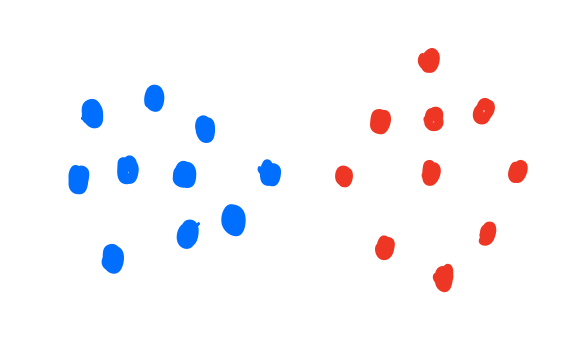
\includegraphics[scale=0.19]{./figs/OPF_Fig17.png} &
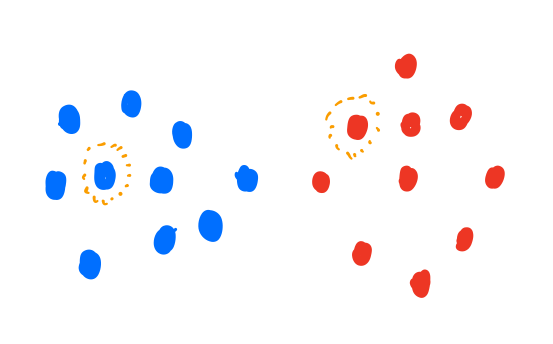
\includegraphics[scale=0.19]{./figs/OPF_Fig18.png} &
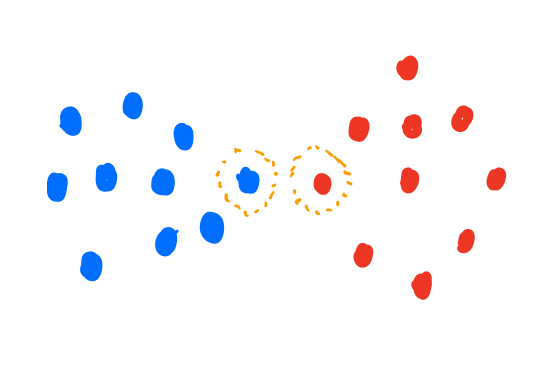
\includegraphics[scale=0.19]{./figs/OPF_Fig19.png}\\
Conjunto de treinamento & Escolha de protótipos & Escolha de protótipos\\
& aleatória & pela MST\\
\end{tabular}
\end{center}
}

\Sli{
Como funciona a escolha de protótipos pela MST? Basicamente, dado o grafo de treinamento e arestas ponderadas pelas distâncias entre os respectivos nós, calculamos a MST e depois selecionamos os nós mais próximos de classes diferentes. Note que temos, ao menos, \textbf{um protótipo para cada classe}, mas nada impede que tenhamos mais.

\begin{center}
\begin{tabular}{ccc}
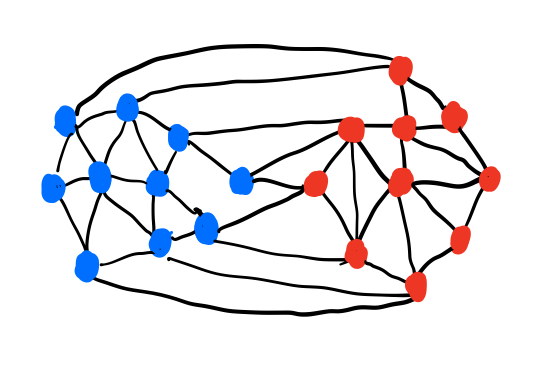
\includegraphics[scale=0.19]{./figs/OPF_Fig20.png} &
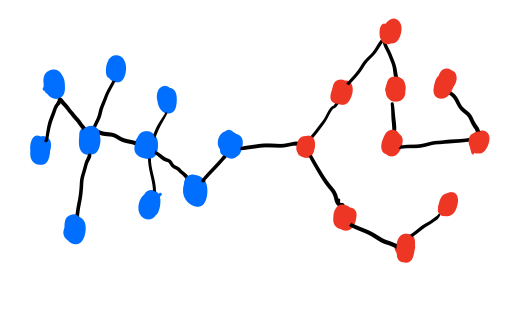
\includegraphics[scale=0.19]{./figs/OPF_Fig21.png} &
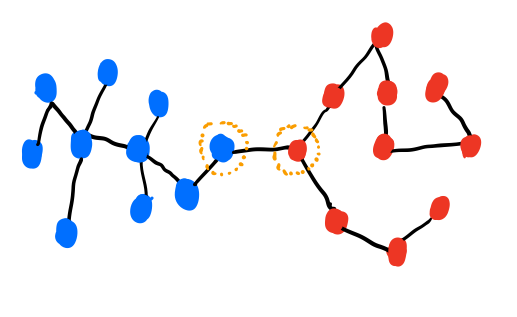
\includegraphics[scale=0.19]{./figs/OPF_Fig22.png}\\
Grafo de treinamento & MST & Protótipos selecionados\\
\end{tabular}
\end{center}
}

\Sli{
Um outro exemplo de situação bastante comum. Note que o classificador OPF possui suporte à classificação por múltiplas de classes de maneira \textbf{nativa}.

\begin{center}
\begin{tabular}{ccc}
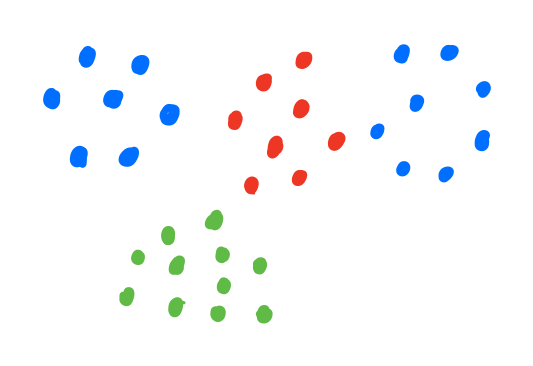
\includegraphics[scale=0.19]{./figs/OPF_Fig23.png} &
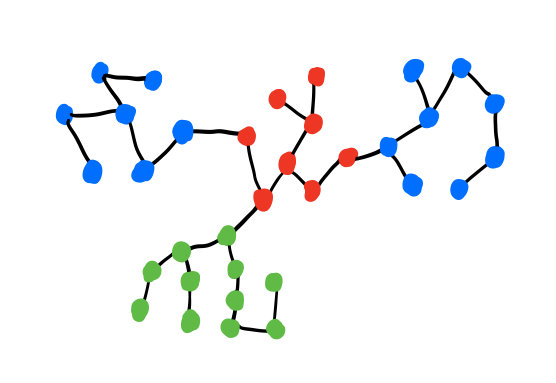
\includegraphics[scale=0.19]{./figs/OPF_Fig24.png} &
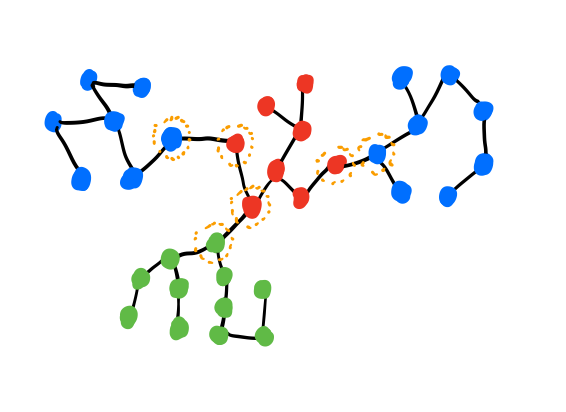
\includegraphics[scale=0.19]{./figs/OPF_Fig25.png}\\
Grafo de treinamento & MST & Protótipos selecionados\\
\end{tabular}
\end{center}
}

\Sli{
\justify Como funciona a função de custo de caminho? Como dito anteriormente, OPF pode trabalhar com diferentes opções para relação de adjacência e metodologia para estimar protótipos. O mesmo ocorre com a função de custo. A versão que veremos faz uso da função de custo definida como segue:

\begin{equation}
	C(\boldsymbol{x}_i)=
\begin{cases}
0\text{ caso $\boldsymbol{x}_i\in{\cal S}$}\\
\infty\text{ caso contrário,}
\end{cases}
\end{equation}
e
\begin{equation}
	C_{\boldsymbol{x}_j}(\boldsymbol{x}_i)=\max\{C(\boldsymbol{x}_j),w(\boldsymbol{x}_j,\boldsymbol{x}_k)\}.
\end{equation}
\justify Neste caso, temos que ${\cal S}$ corresponde ao conjunto de protótipos escolhidos pela MST, $C_{\boldsymbol{x}_j}(\boldsymbol{x}_i)$ corresponde ao custo oferecido pela amostra $\boldsymbol{x}_j$ para a amostra $\boldsymbol{x}_i$ e $w(\boldsymbol{x}_j,\boldsymbol{x}_k)$ denota a distância (peso da aresta) entre os nós $\boldsymbol{x}_j$ e $\boldsymbol{x}_k$, tal que $\boldsymbol{x}_i,\boldsymbol{x}_j,\boldsymbol{x}_k\in{\cal X}^1$.
}

\Sli{
O algoritmo do OPF pode ser entendido como um problema de otimização, em que a ideia é atribuir o \textbf{menor custo possível} à cada amostra de treinamento. Desta forma, a ideia seria resolver o seguinte problema de otimização:

\begin{equation}
C(\boldsymbol{x}_i) = \min\{\max_{\forall \boldsymbol{x}_j\in{\cal X}^1\backslash\{\boldsymbol{x}_i\}}\{C(\boldsymbol{x}_j),w(\boldsymbol{x}_j,\boldsymbol{x}_i)\}\}.
\end{equation}
}

\Sli{
Vejamos um exemplo de funcionamento da etapa de treinamento do algoritmo do OPF.

\begin{center}
\begin{tabular}{ccc}
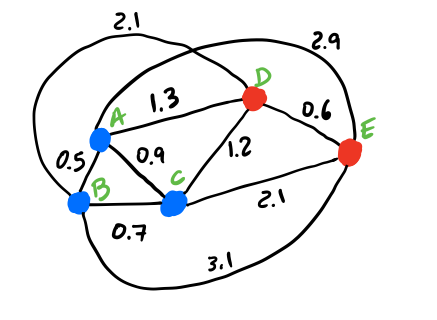
\includegraphics[scale=0.23]{./figs/OPF_Fig26.png} \hspace{3cm}&
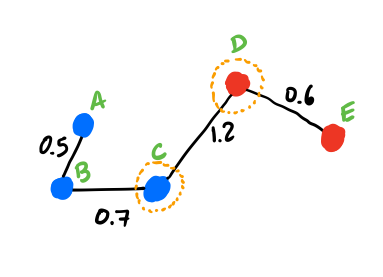
\includegraphics[scale=0.23]{./figs/OPF_Fig27.png} \hspace{3cm}&
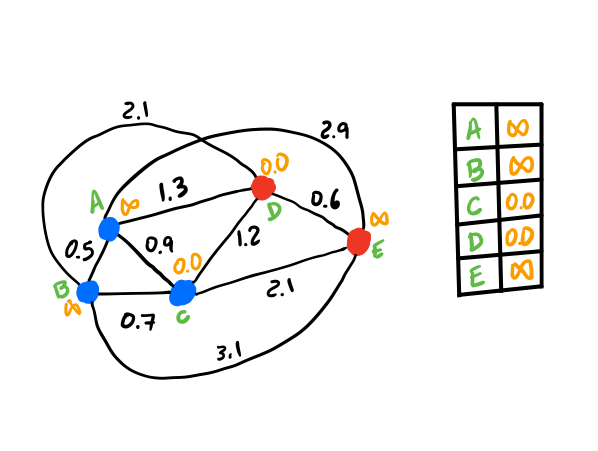
\includegraphics[scale=0.23]{./figs/OPF_Fig28.png}\\
Grafo de treinamento & MST & Inicialização dos custos\\
\end{tabular}
\end{center}
}

\Sli{

\begin{center}
\begin{tabular}{ccc}
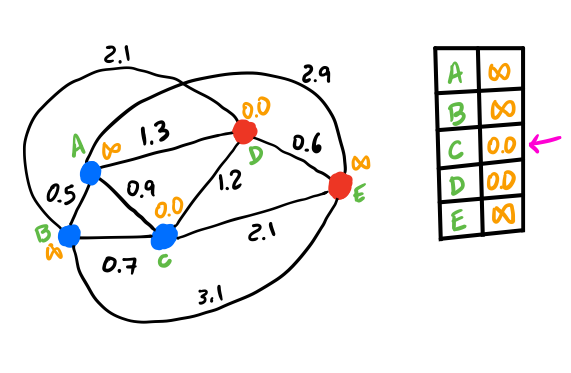
\includegraphics[scale=0.23]{./figs/OPF_Fig29.png} \hspace{3cm}&
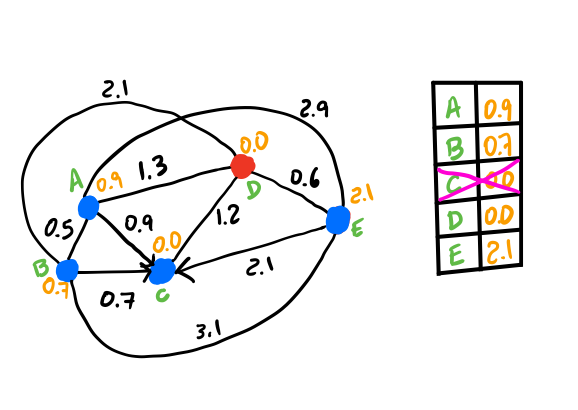
\includegraphics[scale=0.23]{./figs/OPF_Fig30.png} \hspace{3cm}&
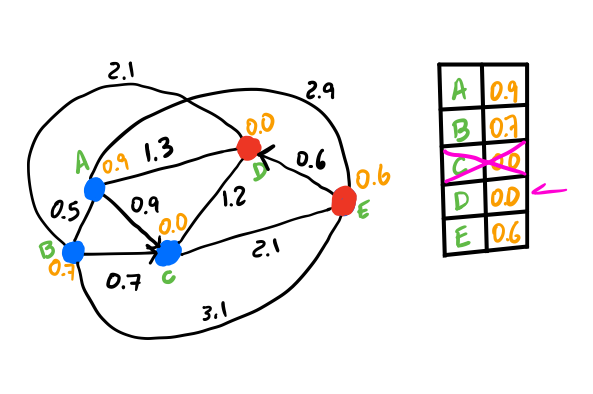
\includegraphics[scale=0.23]{./figs/OPF_Fig31.png}\\
Retirada do protótipo & Custos atualizados & Próximo protótipo\\
da fila de prioridades & & sai da fila\\
\end{tabular}
\end{center}
}

\Sli{

\begin{center}
\begin{tabular}{ccc}
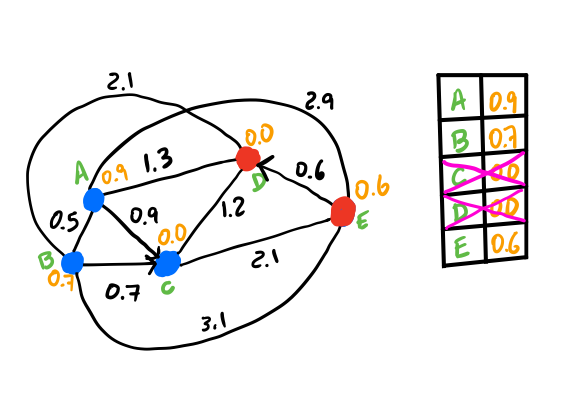
\includegraphics[scale=0.2]{./figs/OPF_Fig32.png} \hspace{3cm}&
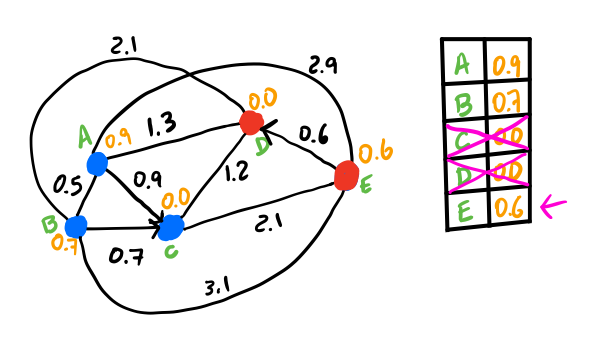
\includegraphics[scale=0.2]{./figs/OPF_Fig33.png} \hspace{1cm}&
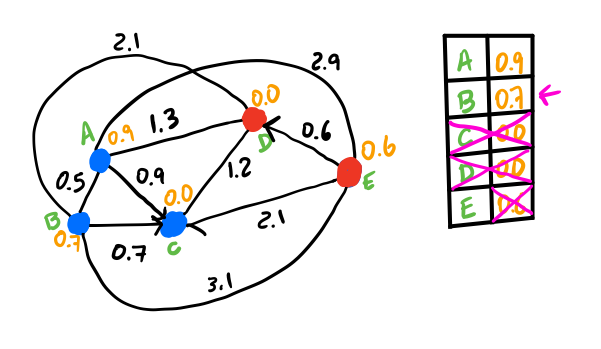
\includegraphics[scale=0.2]{./figs/OPF_Fig34.png}\\
Custos atualizados & Próxima amostra sai & Sem atualização de custo e próxima \\
& da fila de prioridades & amostra sai da fila de prioridades \\
\end{tabular}
\end{center}
}

\Sli{

\begin{center}
\begin{tabular}{ccc}
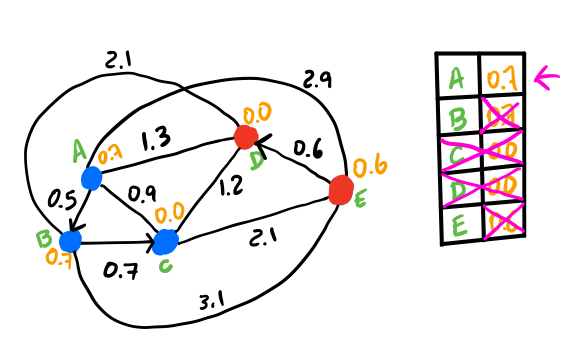
\includegraphics[scale=0.21]{./figs/OPF_Fig35.png} \hspace{3cm}&
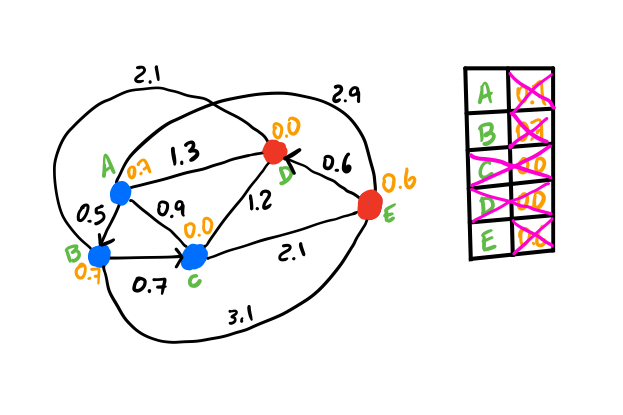
\includegraphics[scale=0.21]{./figs/OPF_Fig36.png} \hspace{1cm}&
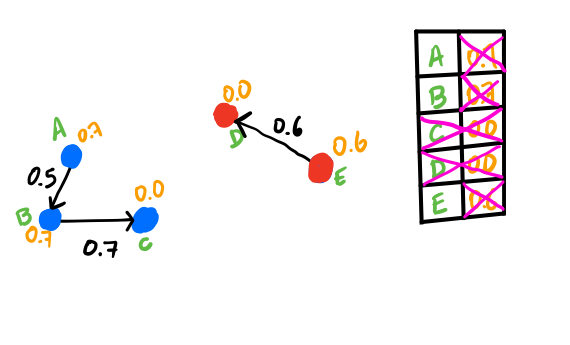
\includegraphics[scale=0.21]{./figs/OPF_Fig37.png}\\
Custos atualizados & Próxima amostra sai & Sem atualização de custo e \\
& da fila de prioridades & fim do treinamento \\
\end{tabular}
\end{center}
}

\Sli{
No final da etapa de treinamento, temos a geração de uma \textbf{floresta de caminhos ótimos}, que é composta por \textbf{árvores de caminhos ótimos} cujas raízes são os nós protótipos. 

\begin{center}
	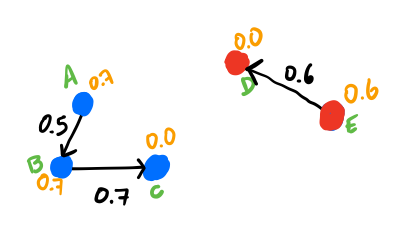
\includegraphics[scale=0.31]{./figs/OPF_Fig38.png}
\end{center}
}

\Sli{
Já a etapa de classificação funciona da seguinte maneira: dada uma amostra $\boldsymbol{x}\in{\cal X}^2$, conectamos ela à todas as amostras do conjunto de treinamento. Em seguida, verificamos quem oferece o melhor custo, de maneira similar à Equação 3, ou seja:

\begin{equation}
C(\boldsymbol{x}) = \min\{\max_{\forall \boldsymbol{x}_i\in{\cal X}^1}\{C(\boldsymbol{x}),w(\boldsymbol{x}_i,\boldsymbol{x})\}\}.
\end{equation}

A amostra $\boldsymbol{x}_i\in{\cal X}^1$ que oferecer o menor custo conquista a amostra de teste e oferece o seu rótulo (classe) à ela.
}

\Sli{
\begin{center}
\begin{tabular}{cc}
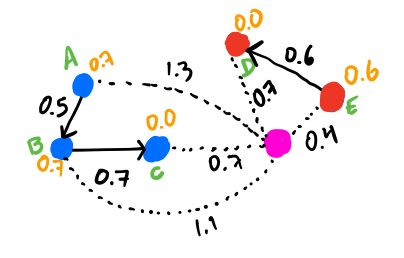
\includegraphics[scale=0.33]{./figs/OPF_Fig39.png} \hspace{3cm}&
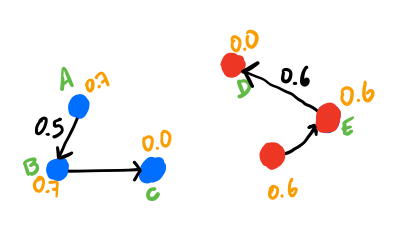
\includegraphics[scale=0.33]{./figs/OPF_Fig40.png} \hspace{1cm} \\
Amostra de teste é conectada à& Amostra recebe o seu \\
todas as amostras de treinamento & rótulo final\\
\end{tabular}
\end{center}
}

\Sli{
\justify O classificador OPF possui outras variantes supervisionadas (OPF com relação de adjacência por $k$-vizinhos mais próximos), semi-supervisionadas e não supervisionadas. Já foi aplicado em diferentes situações, tais como:

\begin{itemize}
	\item Recuperação de imagens (nativo).
	\item Classificação por múltiplos rótulos.
	\item Classificação de imagens (medicina, engenharia e sensoriamento remoto, dentre outras).
	\item Classificação de gêneros musicais.
	\item Classificação de sinais.
	\item Em conjunto com aprendizado em profundidade.
\end{itemize}
}

\end{document}